% !TeX encoding = UTF-8
% @Yongjian.Li 澳門科技大學-畢業論文 LaTeX template-2023

% User's Guide: 
    % https://iihciyekub.github.io/must-thesis-manual
% Github : 
    % https://github.com/iihciyekub/MUST-Thesis
% Overleaf project: 
    % https://www.overleaf.com/read/mjzpcxztzqzv
% chrome 浏览器扩展程序 overleaf s2t/bib2bbl, 下载地址:
    % https://chrome.google.com/webstore/detail/overleaf-s2tbib2bbl/icekiliecbhnockmfkehoebbkmhmapmo?hl=zh-CN
% bib2bbl online: 
    % https://pychat.online/bib2bbl

% 最後更新: 2023-5-08

\documentclass[
    writingLanguage=chinese,
    addPageTitle=on,
    addDeclaration=on,
    addMUSTlog=off,
    printing=off,
    refIndent=on,
    addFigTOC=on,
    addTabTOC=on,
]{.def/must}


% 論文基本信息,必填不能刪除
\def\shool              {Macau University of Science and Technology}
\def\cnTitle            {XXX 銀行(澳門分行)與 XXX 銀行合併之研究}
\def\cnShortTitle       {\cnTitle}% 頁眉顯示的中文論文短題目
\def\enTitle            {The Study on the Relationship between Social Responsibility and Organizational Trust}
\def\enShortTitle       {\enTitle}% 頁眉顯示的英文論文短題目
\def\Name               {我的姓名}% 名稱
\def\StudentNo          {1809853G-BM30-0053}% 學號
\def\Faculty 	        {商學院}% 所在學院
\def\Program 	        {管理學博士學位}% 學位名稱
\def\Major              {商業量化}% 專業名稱
\def\Supervisor	        {李新 副教授}% 指導老師
\def\DateofWriting		{\datea\today}% 設置論文寫作完成時間
\def\DateofDeclaration	{\dateb\today}% 設置論文原創聲明時間
\def\DateofSignature	{2023/06/30}% 設置簽署論文原創聲明的時間
\def\PublicAfterYears   {5}% 設置論文幾年後公開

\begin{document}

\begin{abstract@cn}{關鍵字1、關鍵字1、關鍵字1、關鍵字1、}
本研究採用2009 年至2014 年首度上市的公司279 家為研究樣本,檢驗公司治理與財務績效之關聯性。利用樣本公司上市時的公司治理變數,檢驗公司治理對上市後的會計績效影響與上市後 30 天的市場報酬,再進而依據過去文獻對公司治理變數的論述,以單一指標衡量,依研究對象中位數區分公司治理程度,以及公司治理變數給予不同分數,驗證對財務績效之影響,並比較「有價證券上市審查準則」強化公司治理制度前後之上市公司,在公司治理與財務績效上是否有差異。透過相關分析、T 檢定、迴歸分析,檢驗三大研究假說,實證結果獲得以下主要結論: 

\end{abstract@cn}

\begin{abstract@en}{keyword1、keyword1、keyword1、keyword1、}
This research used 279 companies established between 2009 and 2014 as the
sample, examining the relationship between corporate governance and financial
performance. Corporate governance variable during the time when company
gets started is used to examine the effect of corporate governance on accounting
effectiveness after the company has been on the market, as well as the effect on
the return rate during the first 30 days of the company’s opening. Further
analysis from literature review on corporate governance, using single
measurement, is according to the median of the level of corporate governance
and the rating of corporate governance variable, to cross examine its effect on
financial performance. Also, a comparison of the effect on strengthening
corporate governance using “Stock Exchange Listing Standards” before and
after the company was listed on the stock market on corporate governance and
financial performance. Correlation, T-test, and Regression analysis were used to
examine three hypotheses. Findings include:

1) Company characteristics
High Tech industry has better corporate governance mechanism than traditional
industries.

2) Characteristic of corporate governance level
High corporate governance companies have better accounting effectiveness and
market performance.
\end{abstract@en}

% 添加目錄 
\addtableofcontents

\chapter{緒論}

\section{研究動機與目的}
\citep{luey2013, turabian2015, WangZhenWu2004, WenZaoWai2009, QiuZiHeng2017, HeDingZhao2019, WuPeiHua2020, QiuJiongYou2014, QiuJiongYou2016, QiuJiongYou2019, LinDongTai2008, LinJing2018, LinWenYao2018, LinXHui2014, HongWenQi2019, HongZhenZhou2018, ChenYaNing9999, ChenXiaMin2019, ZhangYan2016, GuoJiaTu2019, WenDaMao2015, JianYiLing2019, bourdieu1990, cohen2007, harvey2007, manguel2009, šteger2010, Villazón2011, bordwell2013, cole2013, deliot2014, foster2017, paige2017, johnson2018, wipawin2018, poff2019, giles2019, TaiwanNews2019, abdoh2019, macdonald2020, Milliot2020, OrganisationforEconomicCo2020, rothfeld2020, crotty2020, melero2021}

\subsection{研究動機}
美 國 學 者 對 公 司 治 理 的 討 論 可 追 溯 自 1930 年代, Berle \&
Means(1932)指出,美國企業存在著股權分散的必要性,因為隨著企業
規模不斷的擴大,使得多數的中大型公司皆需將經營權與所有權加以
分離來經營,以期達到專業化的目的。
有系統地討論此一問題者為Jensen,在1988年Jensen首度有系統地
收錄以公司治理為主題的文章(Weston, Siu \& Johnson; 2002)。亞洲金融
風暴以降,企業美化財務報表、操縱盈餘管理及掏空資產事件層出不
窮,強化公司治理機制遂成為各界關心與注重的現象。公司治理機制
可謂制度面與市場面兩者間所形成的一種組合,被用來作為導引公司
的決策者,在做決策時,能面面俱到地考量各個利害關係人之利益並
且以公司價值之最大化為目標(Denis \& McConnell;2003)。
「公司治理」(Corporate Governance),臺灣學者譯法不一,基於
監督、防弊觀念者有稱之為「公司管控」或「公司監理」,強調興利功
能者則稱之為「公司管理」或「公司統理」;或許各種名詞所界定的意
義與範圍不盡相同,但其主要的內涵均係使企業體透過法律的制衡管
控與設計,在企業所有權與企業經營權分離的組織體系中,能有效監
督組織活動,並且健全組織運作,以防止脫法行為之經營弊端出現,
以實現企業社會責任的目標。
\txtHere[1]

\begin{axiom}
这是公理。
\end{axiom}


\begin{theorem}
这是第二个定理。
\end{theorem}



\begin{definition}
这是定義 definition。
\end{definition}


\begin{example}
这是例子 example。
\end{example}



\begin{property}
这是第二个性質 property。
\end{property}

\begin{proposition}
这是第二个命題 proposition。
\end{proposition}


\begin{lemma}
这是第二个引理 lemma。
\end{lemma}

\begin{corollary}
这是第二个推論 corollary。
\end{corollary}

\begin{remark}
這是註解 remark。
\end{remark}



\begin{condition}
这是條件 condition。
\end{condition}



\begin{conclusion}
这是結論 conclusion。
\end{conclusion}


\begin{assumption}
这是假設 assumption。
\end{assumption}
\section{论文图例}
\captionsetup[figure]{singlelinecheck=off,justification=raggedright}
\captionsetup[subfigure]{singlelinecheck=on}
\tikzstyle{every pin}=[fill=white,draw=black,font=\small,]
\begin{figure}[H]
	\centering
	\begin{subfigure}{0.49\textwidth}
	  	\centering
		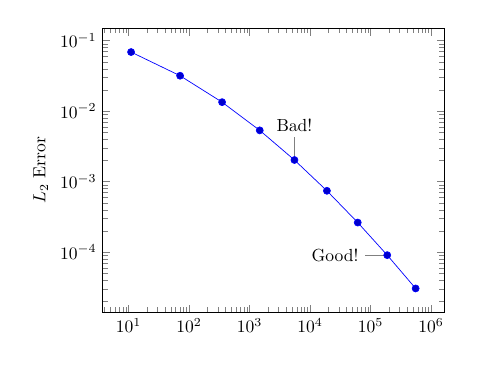
\begin{tikzpicture}[scale = 0.63276]
			\begin{loglogaxis}[
				%xlabel={\textsc{Dof}},
				ylabel={$L_2$ Error},
				]
				\addplot coordinates {
					(11, 6.887e-02)
					(71, 3.177e-02)
					(351, 1.341e-02)
					(1471, 5.334e-03)
					(5503, 2.027e-03)
					(18943, 7.415e-04)
					(61183, 2.628e-04)
					(187903, 9.063e-05)
					(553983, 3.053e-05)
				};
				\node [coordinate,pin=above:{Bad!}]
				at (axis cs:5503,2.027e-03) {};
				\node [coordinate,pin=left:{Good!}]
				at (axis cs:187903,9.063e-05) {};
			\end{loglogaxis}
		\end{tikzpicture}
		\caption{A subfigure}
		\label{fig:sub1}
	\end{subfigure}
	\hfill
	\begin{subfigure}{.49\textwidth}
		\centering
		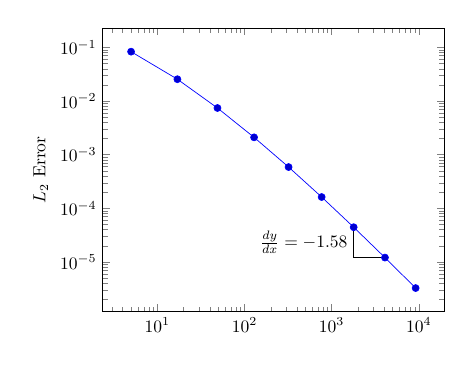
\begin{tikzpicture}[scale = 0.63276]
			\begin{loglogaxis}[
				ylabel=$L_2$ Error,
				]
				\draw
				(1793,4.442e-05)
				|- (4097,1.207e-05)
				node [near start,left]
				{$\frac{dy}{dx} = -1.58$};
				\addplot coordinates {
					(5, 8.312e-02)
					(17, 2.547e-02)
					(49, 7.407e-03)
					(129, 2.102e-03)
					(321, 5.874e-04)
					(769, 1.623e-04)
					(1793, 4.442e-05)
					(4097, 1.207e-05)
					(9217, 3.261e-06)
				};
			\end{loglogaxis}
		\end{tikzpicture}
		\caption{A subfigure}
	  	\label{fig:sub2}
	\end{subfigure}\\

	\begin{subfigure}{.49\textwidth}
		\centering
		
\includegraphics[width=.5\linewidth]{.def/.resource/eg05.png}
		\caption{A subfigure}
		\label{fig:sub3}
	\end{subfigure}
	\begin{subfigure}{.49\textwidth}
		\centering
		
\includegraphics[width=.5\linewidth]{.def/.resource/eg06.png}
		\caption{A subfigure}
		\label{fig:sub4}
	\end{subfigure}
	\caption{A figure with two subfigures}
	\label{fig:sub}
\end{figure}
 
上面示例中,子圖\ref{fig:sub1}、子圖\ref{fig:sub2}、子圖\ref{fig:sub3}、子圖\ref{fig:sub4}分別表示子圖



\section{表}

\captionsetup[table]{singlelinecheck=off,justification=raggedright}
\begin{table}
\caption{這是表的標題}
\centering
\begin{tabularx}{\textwidth}{XXX} % 表格寬度為網頁的一半
\toprule
內容1 & 內容2 & 內容3 \\
\midrule
行1 & 行1 & 行1\footnote{這是表格脚注的內容。} \\
行2 & 行2 & 行2 \\
\bottomrule
\end{tabularx}
\caption*{這是表格脚注}
\end{table}





\subsection{研究目的}

\txtHere[2]

\subsection{研究方法}

本文采用了隨機控制實驗設計,結合問卷調查和實驗數據分析的方法,對研究對象進行了深入的研究。

\subsection{主要貢獻}

\txtHere[3]

\section{相關工作}

本章將介紹相關領域的研究現狀,總結前人的工作成果,分析其不足之處,為後續研究提供理論和實踐基礎。

\subsection{前人工作總結}

\txtHere[4]

\subsection{前人工作不足}

\txtHere[5]

\section{研究內容}

本章將詳細介紹本文的研究內容和研究結果,包括實驗設計、實驗過程、實驗結果分析等。

\subsection{實驗設計}

\txtHere[6]

\subsection{實驗過程}

\txtHere[7]

\subsection{實驗結果分析}

\txtHere[8]

\section{總結和展望}

本章將對本文的研究內容和成果進行總結,並提出未來研究方向和建議。

\subsection{研究總結}

\txtHere[9]

\subsection{未來研究方向}

\txtHere[10]



% 請確保bib 文件名稱為 ref.bib, 利用js文件處理後的bbl文件名稱為 ref.bbl
\addreference


\begin{appendix}
證明過程
\end{appendix}


\begin{acknowpage}
謝謝各位
\end{acknowpage}




% 填寫個人簡歷
\begin{addcvpage}
% 設置入學時間
\addedudate{2019 年 7 月}

% 填寫教育經歷,注意內容以逗號作分隔,
\addeduItem{2009.16-2012.13,中國澳門氹仔島澳門科技大學,商學院}
\addeduItem{2009.16-2012.13,澳門科技大學,商學院}
\addeduItem{2009.16-2012.13,澳門科技大學,商學院}


%增加學術文章
\addpaperItem{ 
    \item 中國澳門氹仔島澳門科技大學1中國澳門氹仔島澳門科技大學1中國澳門氹仔島澳門科技大學1中國澳門氹仔島澳門科技大學1中國澳門氹仔島澳門科技大學1中國澳門氹仔島澳門科技大學1中國澳門氹仔島澳門科技大學1中國澳門氹仔島澳門科技大學,
    \item 中國澳門氹仔島澳門科技大學,
}


% 增加項目
\addprojectItem{
    \item 中國澳門氹仔島澳門科技大學,商學院商學院
    \item  商學院商學院商學院中國澳門氹仔島澳門科技大學,商學院商學院商學院商學院商學院中國澳門氹仔島澳門科技大學,商學院商學院商學院商學院商學院
}
\end{addcvpage}








\end{document}